\documentclass[a4paper,12pt]{article}

\usepackage{cmap}					% поиск в PDF
\usepackage[utf8]{inputenc}
\usepackage[T2A]{fontenc}
\usepackage[english,russian]{babel}
\usepackage[autostyle]{csquotes}
\usepackage{graphicx}
\usepackage{caption}
\usepackage{indentfirst}
\usepackage{listings}
\usepackage{float}
\usepackage[authoryear,round]{natbib}
\usepackage{biblatex}
\usepackage{amsmath,amsfonts,amssymb,amsthm,mathtools} 
\graphicspath{ {images/} }
\author{Казакова Элиза}
\date{\today}
\usepackage[left=2cm,right=2cm,top=2cm,bottom=2cm,bindingoffset=0cm]{geometry}
\newcommand{\anonsection}[1]{\section*{#1}\addcontentsline{toc}{section}{#1}}
\begin{document} % Конец преамбулы, начало текста.
	
	\begin{titlepage}
		\fontsize{12pt}{12pt}\selectfont
		\noindent \begin{minipage}{0.15\textwidth}
			
\includegraphics[width=\linewidth]{ MGTU.png}
		\end{minipage}
		\noindent\begin{minipage}{0.9\textwidth}\centering
			\textbf{Министерство науки и высшего образования Российской Федерации}\\
			\textbf{Федеральное государственное бюджетное образовательное учреждение высшего образования}\\
			\textbf{«Московский государственный технический университет имени Н.Э.~Баумана}\\
			\textbf{(национальный исследовательский университет)»}\\
			\textbf{(МГТУ им. Н.Э.~Баумана)}
		\end{minipage}
		
		\noindent\rule{18cm}{3pt}
		\newline\newline
		\noindent 
		ФАКУЛЬТЕТ 
		\underline{«Информатика и системы управления»} \newline\newline
		
		\noindent КАФЕДРА \underline{«Программное обеспечение ЭВМ и информационные технологии»}\newline\newline\newline\newline\newline\newline\newline
		
		\begin{center}
			\Large\textbf{\qquad\qquad Отчет по лабораторной работе №2} \newline
		\end{center}
		
		\begin{center}
			\textbf{\qquad\qquad       По дисциплине: Анализ Алгоритмов} \newline
		\end{center}
		\textbf{\qquad\qquad\qquad Тема: } \underline{Алгоритмы умножения матриц} \newline\newline\newline
		\textbf{\qquad Студент} \underline{Казакова Э.М.~~~~~~~~~~~~~~~~~~~~~~~~~~~~~~~~~}\newline\newline
		\textbf{\qquad Группа} \underline{ИУ7-56Б~~~~~~~~~~~~~~~~~~~~~~~~~~~~~~~~~~~~~~~~~~~~~~~~~~~~~}\newline\newline
		\textbf{\qquad Оценка (баллы)} \underline{~~~~~~~~~~~~~~~~~~~~~~~~~~~~~~~~~~~~~~~~~~~~~~~~~~~}\newline\newline
		\textbf{\qquad Преподаватели} \underline{Волкова Л.Л., Строганов Ю.В.~~~~~~~~~~}\newline
		
		\begin{center}
			\vfill
			Москва~---~\the\year
			~г.
		\end{center}
	\end{titlepage}
	
	\tableofcontents
	\newpage
	
	\anonsection{Введение}
	\hfill
	
	Цель данной лабораторной работы: провести сравнительный анализ
	алгоритмов умножения матриц и получить навык оптимизации алгоритмов.
	
	Задачи данной лабораторной работы:
	\begin{enumerate}
		\item дать математическое описание формулы расчета для двух алгоритмов: стандартного и алгоритма Винограда
		\item реализовать стандартный алгоритм умножения матриц и алгоритм
		Винограда;
		\item разработать оптимизированый алгоритм Винограда;
		\item дать теоретическую оценку трудоемкости трем алгоритмам;
		\item провести замеры процессорного времени работы реализаций всех трех
		алгоритмов при четных и нечетных размерностях.
	\end{enumerate}

	\newpage
	\section{Аналитическая часть}
	
	\hfill
	
	В данной части будут рассмотрены основные теоретические аспекты, связанные с алгоритмами умножения матриц, описания алгоритмов, формулы и оценки сложностей алгоритмов.
	
	\subsection{Описание классического алгоритма умножения матриц}
	\hfill
	
	\textbf{Матрица} – это прямоугольная таблица каких-либо элементов. Здесь и далее мы будем рассматривать только матрицы, элементами которых являются числа. Упорядоченная пара чисел (n, m), где n - количество строк в матрице, m - количество столбцов, называется размерностью матрицы, обозначается обычно m x n.\\
	Пусть имеются две матрицы: A и B размерами n x l и l x m соответственно.\\
	\[ \begin{bmatrix}
		a_{1,1} & a_{1,2} & ... & a_{1,l} \\
		a_{2,1} & a_{2,2} & ... & a_{2,l}\\		
		... & ... & ... & ... \\
		a_{n,1} & a_{n, 2} & ... & a_{n,l} \\
	\end{bmatrix} \]\\
	\[ \begin{bmatrix}
		b_{1,1} & b_{1,2} & ... & b_{1,m} \\
		b_{2,1} & b_{2,2} & ... & b_{2,m}\\		
		... & ... & ... & ... \\
		b_{l,1} & b_{l, 2} & ... & b_{l,m} \\
	\end{bmatrix} \]\\
	
	
	\textbf{Произведением матриц} A и B размерами n x l и l x m соответственно называется матрица C размерами n x m, каждый элемент которой вычисляется по формуле 1:\\
	\begin{equation}
		c_{i,j} = \sum\limits_{r=1}^n a_{i,r}\cdot b_{r,j}
	\end{equation}		
	\[ \begin{bmatrix}
		c_{1,1} & b_{1,2} & ... & c_{1,m} \\
		c_{2,1} & b_{2,2} & ... & c_{2,m}\\		
		... & ... & ... & ... \\
		c_{n,1} & c_{n, 2} & ... & c_{n,m} \\
	\end{bmatrix} \]\\
	
	
	Матрица C в стандартном алгоритме находится последовательным вычислением элементов с индексами i, j, $i = \overline{1,n}$, $j = \overline{1,m}$ по формуле 1.[1]
	\subsection{Описание алгоритма Винограда}
	\hfill
	
	Если посмотреть на результат умножения двух матриц, то видно,
	что каждый элемент в нем представляет собой скалярное произведение
	соответствующих строки и столбца исходных матриц. Также некоторые вычисления можно произвести заранее, что ускорит выполнение алгоритма.
	Рассмотрим два вектора V = $(v_{1}, v_{2}, v_{3}, v_{4})$ и W = $(w_{1}, w_{2}, w_{3}, w_{4})$\\
	Их скалярное произведение равно\\
	\begin{equation}
		V \cdot W=v_1 \cdot w_1 + v_2 \cdot w_2 + v_3 \cdot w_3 + v_4 \cdot w_4 
	\end{equation}
	Это равенство можно переписать в виде\\
	\begin{equation}
		V \cdot W=(v_1 + w_2) \cdot (v_2 + w_1) + (v_3 + w_4) \cdot (v_4 + w_3) - v_1 \cdot v_2 - v_3 \cdot v_4 - w_1 \cdot w_2 - w_3 \cdot w_4
	\end{equation}\\
	В Алгоритме Винограда используется скалярное произведение из формулы 3, в отличие от стандартного алгоритма.[2] Алгоритм Винограда позволяет выполнить предварительную обработку матрицы и запомнить значения для каждой строки/столбца матриц.
	Над предварительно обработанными элементами нам придется выполнять лишь первые два умножения и последующие пять сложений, а также
	дополнительно два сложения.\\
	\subsection{Вычисление сложности алгоритма}
	\hfill
	
	В рамках данной работы используется следующая модель вычислений:\\
	\begin{enumerate}
		\item базовые операции имеют трудоемкость 1 (<, >, =, <=, =>, ==, +, -, *, /, \%, \&, +=, -=, *=, /=,  [ ]);\\
		\item операторы if, else if имеют трудоемкость $F_{if} = F_{body} + F_{cheсk}$,  $F_{body}$ - трудоемкость операций тела оператора,  $F_{cheсk}$ - трудоемкость проверки условия;\\
		\item оператор else имеет трудоемкость $F_{body}$;\\
		\item оператор for имеет трудоемкость  $F_{for} = 2 + N \cdot (F_{body} + F_{cheсk})$, где $F_{body}$ – трудоемкость операций в теле цикла.\\
	\end{enumerate}

	\newpage
	\section{Конструкторская часть}
	\hfill
	В данном разделе будут рассмотрены схемы алгоритмов умножения матриц: стандартного, Винограда и оптимизированного алгоритма Винограда.
	\subsection{Схемы алгоритмов}
	\hfill
	
	На рисунке 1 представлена схема классического алгоритма умножения
	матриц.
	\begin{figure}[H]
		\centering
		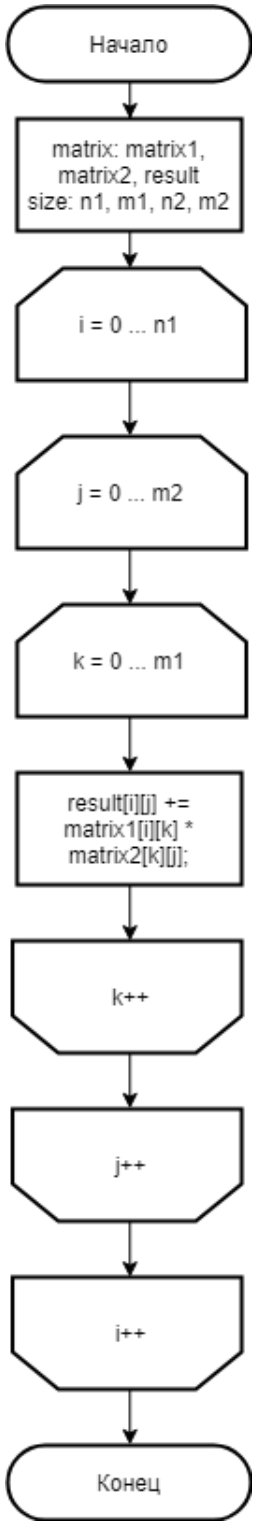
\includegraphics{classic.png}
		\captionsetup{justification=centering}
		\caption{Схема матричного алгоритма нахождения расстояния Левенштейна.}
		\label{Рис 1}
	\end{figure}

	На рисунке 2 представлена схема алгоритма Винограда.
	\begin{figure}[H]
		\centering
		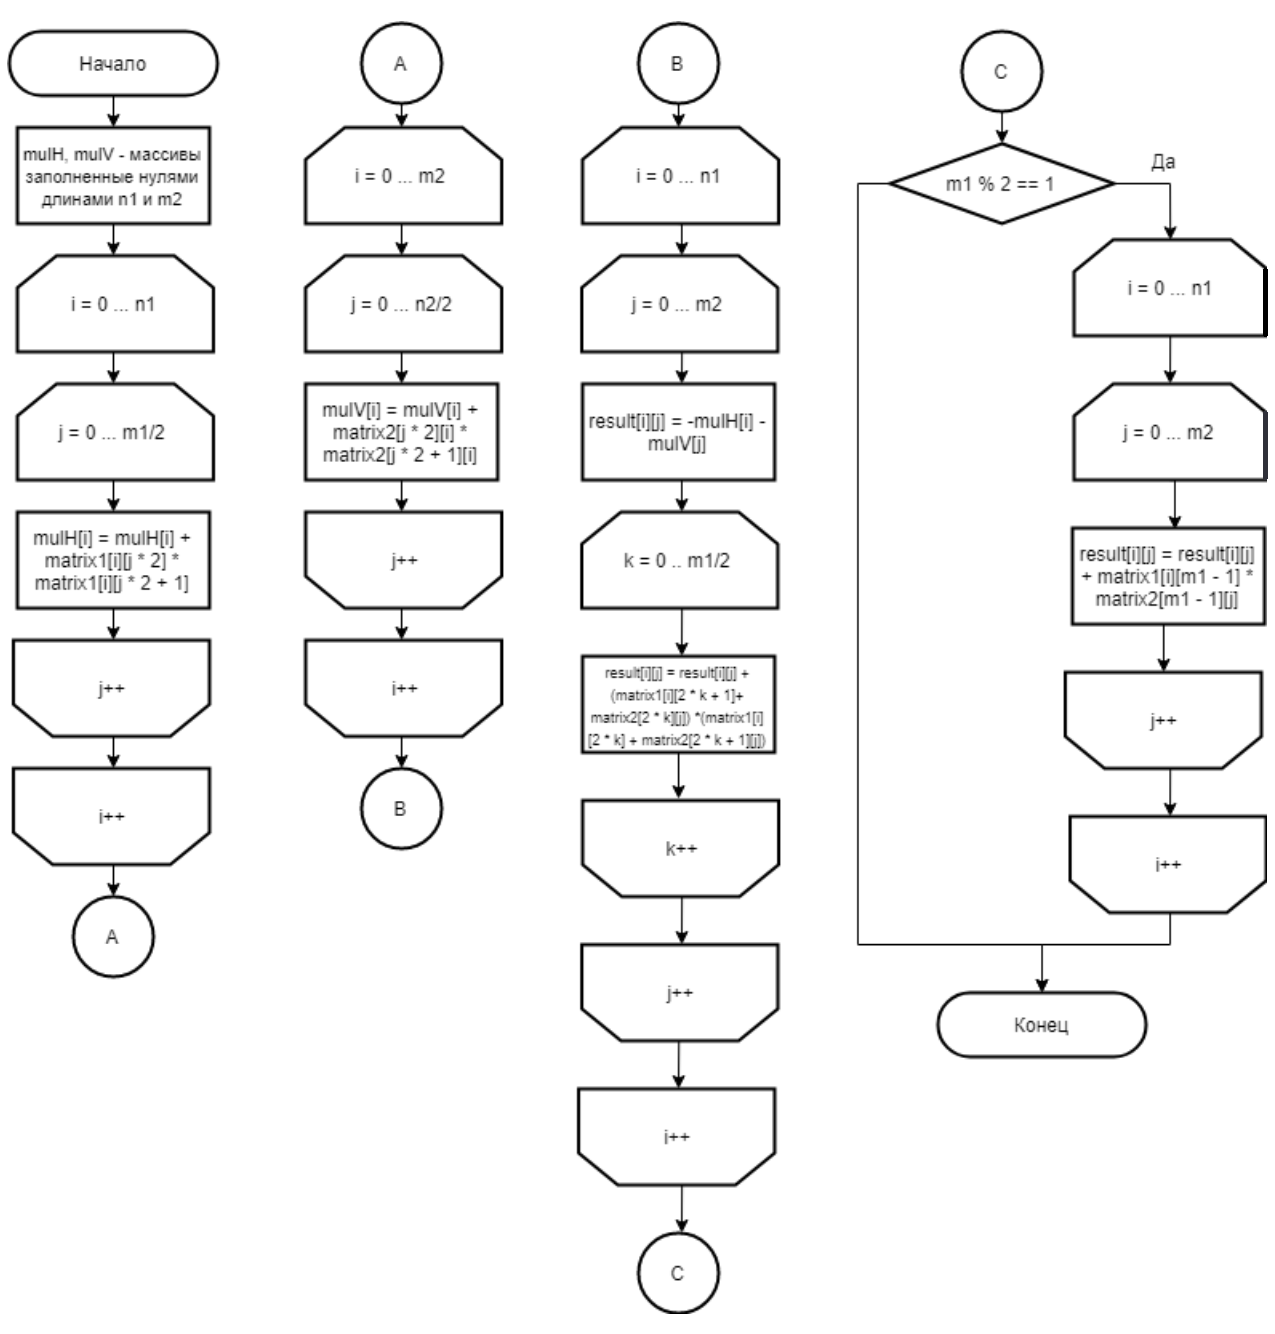
\includegraphics{vinograd.png}
		\captionsetup{justification=centering}
		\caption{Схема рекурсивного алгоритма нахождения расстояния Левенштейна.}
		\label{Рис 2}
	\end{figure}
	На рисунке 3 представлена схема оптимизированного алгоритма Винограда.
	\begin{figure}[H]
		\centering
		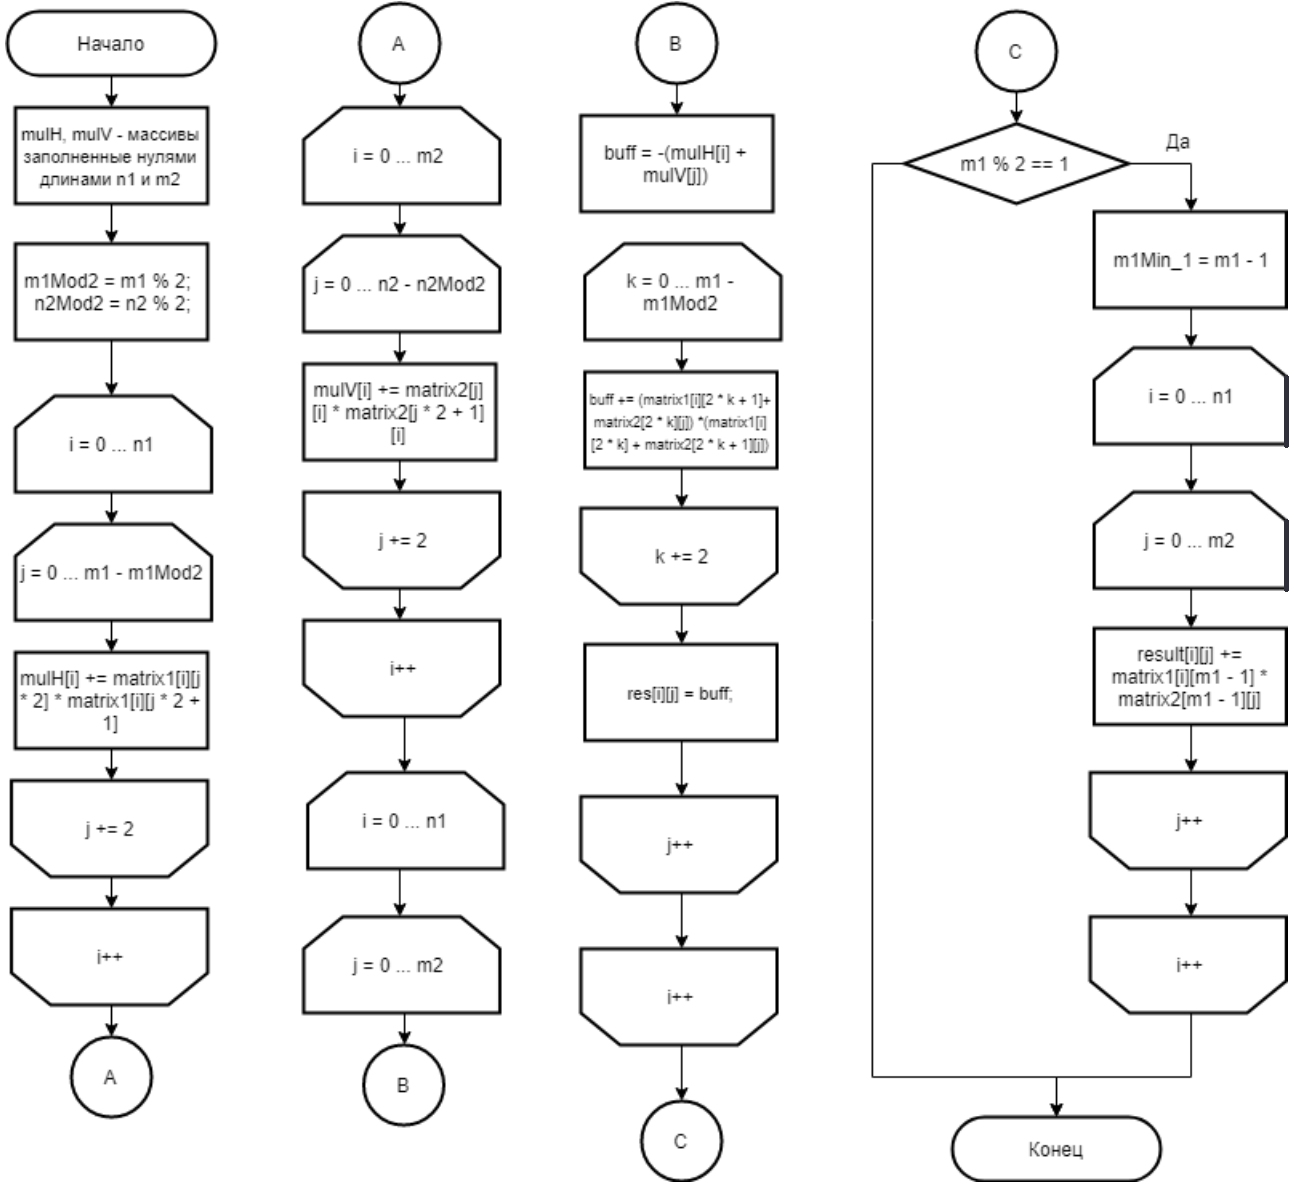
\includegraphics{optimizedvinograd.png}
		\captionsetup{justification=centering}
		\caption{Схема рекурсивного алгоритма нахождения расстояния ДамерауЛевенштейна.}
		\label{Рис 3}
	\end{figure}
	\newpage
	\section{Технологическая часть}
	\hfill
	
	В данном разделе будут рассмотрены требования к программному обеспечению, средства реализации и представлен листинг кода.
	\subsection{Требования к программному обеспечению}
	\hfill
	
	ПО должно предоставлять возможность ввода двух матриц, на выходе пользователь должен получить результат умножения двух матриц, посчитанный тремя алгоритмами. Также ПО должно обеспечить вывод замеров времени работы каждого из алгоритмов.
	
	\subsection{Средства реализации}
	\hfill
	
	В данной работе используется язык программирования Python, так как ЯП позволяет написать программу за кратчайшее время.В качестве среды разработки выбрана IDLE. Для замеров времени была выбран метод process\_time() модуля time[3], он возвращает значение (в долях секунды) системного процессорного времени текущего процесса.
	
	\subsection{Листинг кода}
	\hfill
	
	В листингах 3.1 - 3.3 представлена реализация стандартного алгоритма умножения матриц, алгоритма Винограда и оптимизированного алгоритма Винограда.
	\lstset{ %
		language=Python,                % Язык программирования 
		numbers=left,                   % С какой стороны нумеровать                           
	}
	\textbf{\\Листинг 3.1 -- Стандартный алгоритм умножения матриц}
	
	\begin{lstlisting}
def standart_multiplication_matrix(m1, m2):
	n = len(m1)  
	q = len(m2[0])   
	m = len(m1[0])   
	m3 = [[0] * q for i in range(n)]
	start_time = time.process_time()
	for i in range(0, n):
		for j in range(0, q):
			for k in range(0, m):
				m3[i][j] = m3[i][j] + m1[i][k] * m2[k][j]
	t = time.process_time() - start_time
	return t
	\end{lstlisting}
	\textbf{\\Листинг 3.2 -- Алгоритм Винограда }
	
	\begin{lstlisting}
def vinograd_multiplication_matrix(m1, m2):
	m = len(m1)   
	n = len(m1[0])   
	q = len(m2[0]) 
	m3 = [[0] * q for i in range(m)]
	
	row = [0] * m
	for i in range(0, m):
		for j in range(0, n // 2, 1):
			row[i] = row[i] + m1[i][2 * j] * m1[i][2 * j + 1]
	
	col = [0] * q
	for j in range(0, q):
		for i in range(0, n // 2, 1):
			col[j] = col[j] + m2[2 * i][j] * m2[2 * i + 1][j]
	
	start_time = time.process_time()
	for i in range(0, m):
		for j in range(0, q):
			m3[i][j] = -row[i] - col[j]
			for k in range(0, n // 2, 1):
				m3[i][j] = m3[i][j] + 
				     + (m1[i][2 * k + 1] + m2[2 * k][j])*
				     * (m1[i][2 * k] + m2[2 * k + 1][j])
	
	if n % 2 == 1:
		for i in range(0, m):
			for j in range(0, q):
				m3[i][j] = m3[i][j] + 
				           + m1[i][n - 1] * m2[n - 1][j]       
	t = time.process_time() - start_time
	return t
	\end{lstlisting}
	
	\textbf{\\Листинг 3.3 -- Оптимизированный алгоритм Винограда}
	
	\begin{lstlisting}
def vinograd_optimizate_multiplication_matrix(m1, m2):
	m = len(m1)
	n = len(m1[0])
	q = len(m2[0])
	m3 = [[0] * q for i in range(m)]
	row = [0] * m
	for i in range(0, m):
		for j in range(1, n, 2):
			row[i] -= m1[i][j] * m1[i][j - 1]
	
	col = [0] * q
	for j in range(0, q):
		for i in range(1, n, 2):
			col[j] -= m2[i][j] * m2[i - 1][j]
	
	flag = n % 2
	start_time = time.process_time()
	for i in range(0, m):
		for j in range(0, q):
			m3[i][j] = row[i] + col[j]
			for k in range(1, n, 2):
				m3[i][j] += (m1[i][k - 1] + m2[k][j]) *
				* (m1[i][k] + m2[k - 1][j])
			if (flag):
				m3[i][j] += m1[i][n - 1] * m2[n - 1][j]
	t = time.process_time() - start_time
	return t
	\end{lstlisting}
	
	\subsection{Тестирование}
	\hfill
	
	На рисунке 4-5 показаны результаты работы программы при разных входных данных.
	
	\begin{figure}[H]
		\centering
		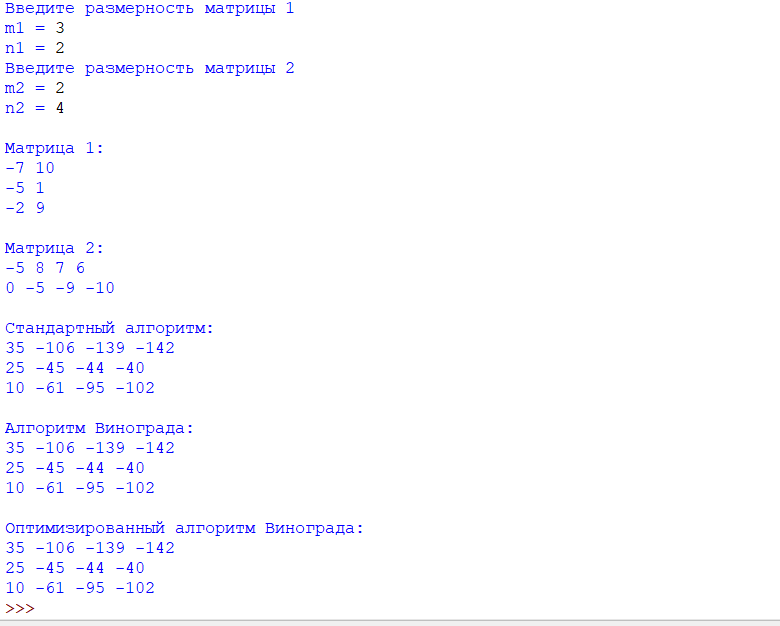
\includegraphics[scale=0.6]{res.png} 
		\captionsetup{justification=centering}
		\caption{Работа программы при умножении матриц c корректными размерами}
		\label{пример1}
	\end{figure}

	\begin{figure}[H]
		\centering
		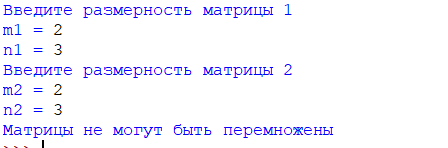
\includegraphics[scale=0.6]{res1.png} 
		\captionsetup{justification=centering}
		\caption{ Работа программы при некорректном задании размеров матрицы}
		\label{пример2}
	\end{figure}
	
    \subsection{Выводы}
    \hfill
    
    В данном разделе была представлена реализация алгоритмов стандартного умножения матриц, Винограда, а также оптимизированного алгоритма Винограда  Программа корректно сработала на вводе матриц с размерами, которые не позволяют перемножить матрицы.
    
    \newpage

	\section{Экспериментальная часть}
	\hfill
	
	В данной части производится экспериментальное сравнение работы трех реализованных алгоритмов (зависимость времени выполнения от размеров матриц и четности/нечетности размеров).
	\subsection{Постановка эксперимента}
	\hfill
	
	В рамках данной лабораторной работы были проведены следующие эксперименты: 
	\begin{enumerate} 
		\item Сравнение времени работы алгоритмов при четном и нечетном размере
		матрицы
	\end{enumerate} 
	\subsection{Сравнение времени работы}	
	\hfill
	
	На графиках 6-7 представлено сравнение времени работы алгоритма на матрицах разных размеров.Матрицы заполняются случайно сгенерированными числами в диапазонеот -10 до 10. Для построения графика на рисунке 6 генерировались матрицы четной размерности. Для построения графика на рисунке 7 генерировались матрицы нечетной размерности.
	
	\begin{figure}[H]
		\centering
		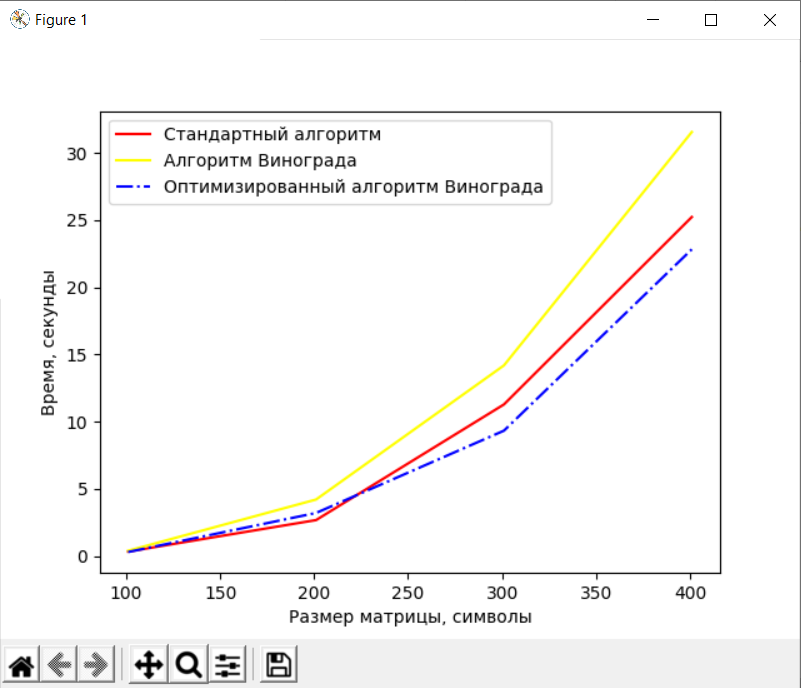
\includegraphics[scale=0.6]{exp1.png} 
		\captionsetup{justification=centering}
		\caption{Сравнение по времени работы реализации алгоритмов нахождения произведения матриц при четных размерностях}
		\label{тест1}
	\end{figure}
	
	\begin{figure}[H]
		\centering
		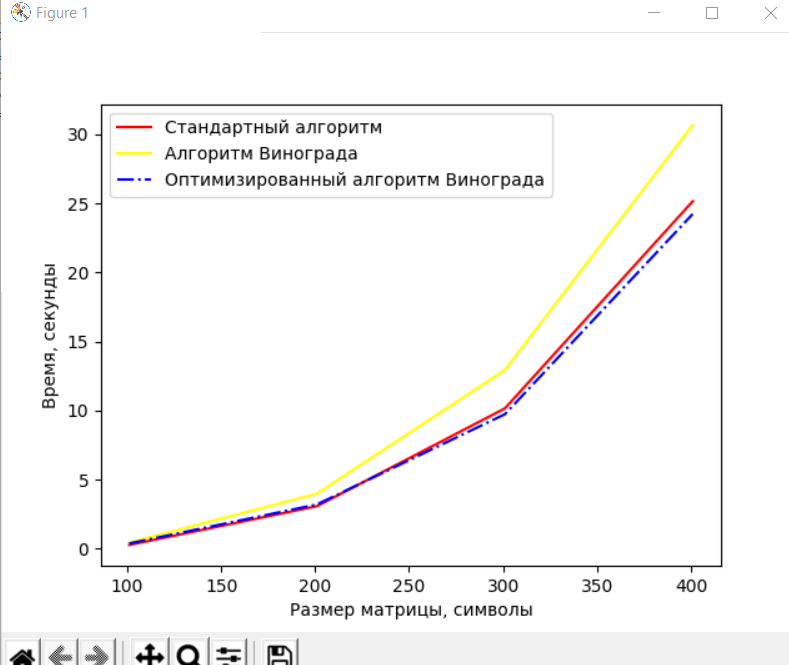
\includegraphics[scale=0.6]{exp2(nechetn).png} 
		\captionsetup{justification=centering}
		\caption{ Сравнение по времени реализации алгоритмов нахождения произведения матриц при нечетных размерностях}
		\label{тест2}
	\end{figure}
	
	
	\subsection{Оценка трудоемкости алгоритмов умножения матриц}
	\hfill
	
	Оценим трудоемкость стандартного алгоритма умножения матриц, алгоритма Винограда и оптимизированного алгоритма Винограда.
	 \begin{enumerate}
		\item Стандартный алгоритм
		$$f=2+M(2+2+Q(2+2+N(2+8+1+1+1)))=13 \cdot MNQ+4MQ+4M+2 \approx 13 \cdot MNQ$$ 
		
		\item Алгоритм Винограда
		
		Трудоемкость алгоритма Винограда:\\
		
		Первый цикл: $\frac{15}{2} \cdot N  Q + 5 \cdot M + 2$ \\
		
		Второй цикл: $\frac{15}{2} \cdot M  N + 5 \cdot M + 2$\\
		
		Третий цикл: $13 \cdot M  N Q + 12 \cdot M Q + 4 \cdot M + 2$\\
		
		Условный переход: $\begin{bmatrix}
			2    &&, {лучший случай (при четном N)}\\
			15 \cdot QM + 4 \cdot M + 4 &&, {худший случай}\\
		\end{bmatrix} $ \\
		
		Итого: $f = \frac{15}{2} \cdot M  N + \frac{15}{2} \cdot Q  N + 9 \cdot M + 8 +  5 \cdot Q + 13 \cdot M  N Q + 12 \cdot M Q 
		+
		\begin{bmatrix}
			2, \text{в лучшем случае}\\
			15 \cdot QM + 4 \cdot M + 4,\text{в худшем}\\
		\end{bmatrix} $ \\
		
		$$f \approx 13 \cdot MNQ $$
		
		\item Оптимизированный алгоритм Винограда
		
		Введем оптимизации: 
		\begin{enumerate}
			\item замена оперции = на += или -=
			\item избавление от деления в условиях цикла (j < N, j += 2)
			\item Заносим проверку на нечетность кол-ва строк внутрь основных циклов
			\item Расчет условия для последнего цикла один раз, а далее использование флага
		\end{enumerate}
		
		Первый цикл: $4 \cdot N  Q + 4 \cdot M + 2$ \\
		
		Второй цикл: $4 \cdot M  N + 4 \cdot M + 2$\\
		
		Третий цикл: $9 \cdot M  N Q + 10 \cdot M Q + 4 \cdot M + 2$\\
		
		Условный переход: $\begin{bmatrix}
			2   &&, \text{лучший случай (при четном N)}\\
			10 \cdot QM &&, \text{худший случай}\\
		\end{bmatrix} $ \\
		
		Трудоемкость оптимизированного алгоритма Винограда:\\
		
		Итого: $$f = 4 \cdot N  Q + 4 \cdot M + 2 + 4 \cdot M  N + 4 \cdot M + 2 + 9 \cdot M  N Q + 10 \cdot M Q + 4 \cdot M + 2 + \begin{bmatrix}
			2   &&, \text{л.c}\\
			10 \cdot QM &&, \text{х.c}\\
		\end{bmatrix} \approx 9 \cdot MNQ$$
		
		
	\end{enumerate}
	
	\subsection{Выводы}
\hfill

	Оптимизированный алгоритм Винограда работает быстрее классического метода и значительно быстрее обычного алгоритма Винограда. 
	
	Несмотря на сложность алгоритма Винограда по сравнению со стандартным, доля умножения в алгоритме Винограда меньше. Также, стоит обратить внимание на то, что при работе алгоритма Винограда с матрицами нечетной размерности, необходимо произвести дополнительные действия, в то время как алгоритм стандартный не зависит от четности размерности матриц.
	
	\newpage
	
	\anonsection{Заключение}
	\hfill
	
	В ходе лабораторной работе были исследованы алгоритмы умножения матриц: стандартный, Винограда и оптимизированный алгоритм Винограда.
	При выполнении лабораторной работе цель была достигнута: был проведен сравнительный анализ алгоритмов умножения матриц и получен навык оптимизации алгоритмов.
	Также были выполнены следующие задачи: 
	
	\begin{enumerate}
		\item были описаны формулы расчета для двух алгоритмов: стандартного и алгоритма Винограда; 
		\item были реализованы стандартный алгоритм умножения матриц и алгоритм Винограда;
		\item был разработан оптимизированый алгоритм Винограда;
		\item посчитана теоретическая оценка трудоемкости трех алгоритмов;
		\item проведены замеры процессорного времени работы реализацийч трех алгоритмов при четных и нечетных размерностях;
	\end{enumerate}

	При сравнении данных алгоритмов пришли к выводу, что классический алгоритм в является более эффективным чем алгоритм Винограда, однако после ряда оптимизаций, алгоритм Винограда становится значительно быстрее стандартного.
	
	\newpage
	 \begin{thebibliography}{}
		
		\bibitem{} Умножение матриц [Электронный ресурс]. - Режим доступа: https://habr.com/ru/post/359272/(дата обращения: 22.01.2021)
		
		\bibitem{} Алгоритм Винограда [Электронный ресурс]. - Режим доступа: https://www.gyrnal.ru/statyi/ru/1153/ (дата обращения: 22.01.2021)
		
		\bibitem{} Златопольский Д.М. Основы программирования на языке Python. – М.: ДМК Пресс, 2017. – 284 с.
	\end{thebibliography} 
	
\end{document} % Конец текста.

